\chapter{QRAcc: A Hybrid DNN Accelerator codesigned for MARP}

\label{chap:qracc}

We discussed in Chapter \ref{section:TinyML} that the MLPerfTiny models are representative of DNNs that are designed for the edge due to their small memory footprint. Since we're targeting these models, we need an accelerator that can run the depthwise convolutions present in them efficiently.

In line with the hybrid accelerator works DIANA \cite{houshmand2022diana} and Garofalo et al. \cite{garofalo2022heterogeneous}, we also forgo mapping depthwise convolutions to AIMC cores entirely and instead map them to a weight-stationary digital accelerator by implementing a heterogenous accelerator containing both an AIMC core and a weight-stationary digital accelerator. The digital accelerator is used to map the depthwise convolutions while the AIMC core is used to map the rest of the DNN layers. We call this heterogenous accelerator QRAcc. QRAcc is designed to support high utilization mappings of modern DNNs with depthwise convolutions. The RTL (digital) parts of QRAcc are available in the repository https://github.com/Lawrence-lugs/QrAccelerator.

Additionally, MARP's rectangular packing schemes (discussed in Chapter \ref{chapter:marp}) for matrix mapping onto AIMCs requires arbitrary X and Y offsets in the mapped matrix in the AIMC memories. To this end, we experimented multiple existing feature loading schemes for AIMC like the ones from the UNPU \cite{lee2018unpu}, NeuRRAM \cite{wanneurram}, and Garofalo 2022 \cite{garofalo2022heterogeneous} and found that none of their schemes allow for arbitrary offsets in the mapped matrix (it is unclear if the controller is able to do so). This creates a need for an AIMC accelerator that can support arbitrary offsets in the mapped matrix.

\section{QRAcc Architecture}

\begin{figure}[h]
    \centering
    \includesvg[width=\linewidth]{images/qracc/qracc_architecture.svg}
    \caption{QRAcc Architecture}
    \label{fig:qracc_architecture}
\end{figure}

In alignment with the motivations above, we designed QRAcc with the following features:

\begin{enumerate}
    \item QRAcc is a hybrid DNN accelerator able to perform quantized linear matrix convolutions of any kernel size and 3x3 depthwise convolutions. When paired with MARP, it's designed to be able to run most modern DNN models end-to-end with the help of a general-purpose processor and large memory.
    \item QRAcc is codesigned to support MARP with the ability to align row inputs and column outputs to the mapped matrix in the AIMC memory array. QRAcc enables the row input alignment required by MARP using a regfile-based feature window loading technique. The output aligner accounts for the column output alignment at the end by changing the addressing scheme into the PISO write queue. 
    \item QRAcc allows reconfigurability and monitoring via control and status registers (CSRs) and memory-mapped addressing, enabling it to be tightly coupled to a processor core over a simple data bus with a valid/ready handshake.
    \item QRAcc utilizes a core MVM accelerator "SeqAcc" for regular convolutions running at SOTA-level 516.1 TOPS/W energy efficiency. SeqAcc improves over previous charge-redistribution SRAM AIMC accelerators \cite{jiang2020c3sram} and is described in detail in Section \ref{section:seqacc}.
    \item Supports true end-to-end integer-only inference of a model via integer-only operations via the output scaling and bias adding per the TensorFlow Lite full-integer quantization implementations \cite{jacob2018quantization}. This is important to enable the use of integer-only processor cores to run the models on the edge.
\end{enumerate}

QRAcc utilizes several blocks to fully implement successive layers of integer-only convolutions and matrix multiplications. The blocks, as shown in Figure \ref{fig:qracc_architecture}, are as follows:

\begin{enumerate}
    \item SeqAcc, the core MVM accelerator which takes in 256-bit vectors and multiplies them with a 256x256 matrix to produce a 256-bit output. We based SeqAcc on significant improvements over C3SRAM, as described in its own section \ref{section:seqacc}.
    \item WSAcc, the weight-stationary depthwise convolution accelerator. We designed WSAcc to be able to share the feature loader (FL) with SeqAcc while at the same time keeping its production bandwidth (the rate at which it produces output data) low enough not to overwhelm the ACTMEM's input bandwidth. 
    \item The local activation memory (ACTMEM), a 256kB memory bank with 2 write ports and 2 read ports. 
    \item The feature loader (FL), a 256B register file with masking functionality and a flexible feature loading technique supporting any kernel shape for convolutions.  
    \item The output processing block aligns the output of SeqAcc for writing into the write queue and performs the rest of the necessary operations (fixed-point multiply, shifts, adds) involved in a QLinearConv.
    \item The write queue stores write the output feature map write requests for the ACTMEM until the ACTMEM is ready. The queue allows SeqAcc to have a different output bandwidth than the activation memory.
    \item The CSRs allow an external processor to configure the QRAcc system and initiate load, readout, or computation. Details on using the CSRs and configuration registers can be found in Appendix \ref{section:qracc_csrs}.
\end{enumerate}

\subsubsection{Activation Memory}

The ACTMEM uses pointers keeps track of flexible locations for the input feature map (IFMAP) and the output feature map (OFMAP). Tracking these pointers enables continuous use of the DNN accelerator for successive layers (ping-ponging) without the need to stream out data. By simply putting the IFMAP pointer into the position of the current OFMAP pointer, the current OFMAP can be turned into the input for the next convolution (\ref{fig:imc_qrAccConvSchem}). The ACTMEM features 2 write ports (one 32 bit for the data bus, one 256-bit from the write queue) and 2 read ports (one 32-bit for the data bus, one 256-bit from the write queue). In the next iteration, we plan to reduce this to a single dual-port SRAM with FIFO queues on all ports.

\subsubsection{Feature Loader}

Combined with a window controller and configuration, the FL can perform an Im2Col transformation to enable $K\times C\times F_X\times F_Y$ convolutions for QRAcc. As shown in Figure \ref{fig:imc_qrAccConvSchem}, the FL manages reads from the ACTMEM in such a way that performs the Im2Col transformation in the fewest reads needed. Because the ML workloads mapped onto SeqAcc are not always MVM to a subset of the SeqAcc rows, the FL masks the data it sends toward the SeqAcc IMC in order to limit the operation to a specific subset of rows. 

\subsubsection{Output Processing}

The output processing block has two jobs: to align the SeqAcc outputs to the write queue, and to perform the scaling and biasing necessary for a QLinearConv. The TFLite paper \cite{jacob2018quantization} contains more details on all the necessary operations.

QLinearConv operations require a fixed-point scaling computation uniformly applied over all elements of the output $y_o$ \cite{jacob2018quantization}. This scaling factor $S_O\in[0,1]$ is typically expressed in fixed-point form such that it splits into a shift and an integer multiplication:

\begin{equation}
    S_0=M_0\times2^S
\end{equation}

where $S$ is a number of shifts typically less than 8 (for 8b x 8b MACs, less shifts for lower precision) and $M_0$ is a 16-bit integer portion of the fixed point scaling factor. Performing this entire operation in hardware requires both a shift and a multiply (as with fixed-point multiplication).

Other than this, a QLinearConv entails two lumped biasing steps that need to be performed: one from before the scaling and one after the scaling. Before scaling, the bias contributions of the batchnorm must be added to the MAC output. After scaling, the offset contributions of the quantization zero points must also be added to the elements.

Finally, the output processing stage saturates the output between $[0,2^n-1]$ where $n$ is the configured number of output bits before passing the output to the write queue.

For exact details on the computation of QLinear operations, refer to the appendix \ref{section:qlinearops}.

\begin{figure}[h]
    \centering
    \includesvg[width=\linewidth]{images/qracc/imc_qrAccConvSchem.svg}
    \caption{Schematic of QRAcc performing a 2x2 convolution with 3 input channels and 5 output channels}
    \label{fig:imc_qrAccConvSchem}
\end{figure}

\subsection{Using QRAcc}

QRAcc supports integer-only convolutions and matrix multiplications. For matrix multiplications, MARP maps them as equivalent 1x1 (pointwise) convolutions. For convolutions, QRAcc supports any kernel size and 3x3 depthwise convolutions. The depthwise convolutions are mapped to the WSAcc block while the rest of the convolutions are mapped to SeqAcc.

\subsubsection{Triggers and CSRs}

CSRs are used for primary control of the accelerator, including triggering operations and monitoring status. Importantly, QRAcc commands are issued by writing the 4b trigger value into main control CSR. The CSRs are memory-mapped, allowing an external processor to configure the QRAcc system and initiate load, readout, or computation. The CSRs are:

\begin{enumerate}
  \item CSR 0: Main Control Register, which contains the main control bits for the QRAcc controller.
  \item CSR 1: Layer Configuration Register, which contains the layer configuration bits for the QRAcc controller.
  \item CSR 2: Input Feature Map Dimension Register, which contains the input feature map dimensions.
  \item CSR 3: Output Feature Map Dimension Register, which contains the output feature map dimensions.
  \item CSR 4: Channel Configuration Register, which contains the number of input and output channels.
  \item CSR 5: Mapped Matrix Offset Register, which contains the X and Y offsets of the mapped matrix in the AIMC memory array.
  \item CSR 6: Padding Information Register, which contains the padding information for the convolution operation.
\end{enumerate}

\begin{longtable}{@{}llll@{}}
\caption{CSR 0: Main Control Register Bit Fields} \\
\toprule
Bits & Field Name & R/W & Description \\ \midrule
\endfirsthead
\multicolumn{4}{c}%
{{\bfseries \tablename\ \thetable{} -- continued from previous page}} \\
\toprule
Bits & Field Name & R/W & Description \\ \midrule
\endhead
\bottomrule
\endfoot
\endlastfoot
2:0 & \texttt{csr\_main\_trigger} & W & Main trigger for the controller. See Table \ref{tab:triggers}. \\
3 & \texttt{csr\_main\_clear} & W & Clears the controller state. \\
4 & \texttt{csr\_main\_busy} & R & Indicates if the controller is not in the idle state. \\
5 & \texttt{inst\_write\_mode} & W & Set to 1 if writing instructions for the microcode loop. \\
11:8 & \texttt{internal\_state} & R & The internal state of the controller FSM for debugging. \\
12 & \texttt{preserve\_ifmap} & W & If set, the input feature map is preserved after computation. \\
\end{longtable}

\begin{longtable}{@{}lll@{}}
\caption{QRAcc Command Triggers} \label{tab:triggers} \\
\toprule
Trigger Name & Value & Description \\ \midrule
\endfirsthead
\multicolumn{3}{c}%
{{\bfseries \tablename\ \thetable{} -- continued from previous page}} \\
\toprule
Trigger Name & Value & Description \\ \midrule
\endhead
\bottomrule
\endfoot
\texttt{TRIGGER\_IDLE} & 0 & No trigger. \\
\texttt{TRIGGER\_LOAD\_ACTIVATION} & 1 & Loads activations into the ACTMEM. \\
\texttt{TRIGGER\_LOADWEIGHTS} & 2 & Loads weights into SeqAcc. \\
\texttt{TRIGGER\_COMPUTE\_ANALOG} & 3 & Starts an analog computation cycle. \\
\texttt{TRIGGER\_COMPUTE\_DIGITAL} & 4 & Starts a digital computation cycle. \\
\texttt{TRIGGER\_READ\_ACTIVATION} & 5 & Reads activations from the ACTMEM. \\
\texttt{TRIGGER\_LOADWEIGHTS\_DIGITAL} & 6 & Loads weights into WSAcc. \\
\texttt{TRIGGER\_LOAD\_SCALER} & 7 & Loads scaler and bias values. \\
\end{longtable}

Figure \ref{fig:imc_qrAccConvSchem} shows an example of QRAcc performing a 2x2 convolution with 3 input channels and 5 output channels. A processor can instruct QRAcc to perform a convolution in a sequence of steps as follows: 

\begin{enumerate}
    \item The processor configures the layer parameters by writing to the CSRs from 0-6. This includes the IFMAP and OFMAP dimensions, the number of input and output channels, the kernel size, the padding information, and the X and Y offsets of the mapped matrix in the AIMC memory array.
    \item The processor initiates a weight load by writing a trigger to CSR 0. QRAcc loads the weights from the external bus into SeqAcc. This step is skipped if the layer's bin (that is, a mapped matrix from MARP) is the same as the current bin inside SeqAcc. For more details on the binning process, refer to Chapter \ref{chapter:marp}.
    \item The processor initiates an input feature map load by writing a trigger to CSR 0. QRAcc loads the input feature map (IFMAP) into the ACTMEM via the external bus. This step is skipped if the IFMAP is already loaded in the ACTMEM which happens when it's the output of the previous layer or an IFMAP is reused for multiple subsequent layers.
    \item The processor initiates either a SeqAcc or WSAcc computation by writing a trigger to CSR 0. QRAcc loads a window of the ifmap into FL while accounting for convolution padding. Typically, this loading step takes 3 cycles (1 for each $F_Y$), but can take more than 3 if $CF_X > 32$, which is the highest number of elements the ACTMEM can provide with its internal interface bandwidth.
    \item SeqAcc (for regular convolutions) or WSAcc (for depthwise convolutions) consumes the data inside the FL and passes it through the QR-based SRAM IMC. After $B_{in}+3$ cycles, where $B_{in}$ is the number of input bits, SeqAcc and WSAcc both can produce $K$ 16b outputs where $K$ is the number of output channels. At most, SeqAcc can support $K=256$ 16b outputs at a time while WSAcc can support $K=32$ 16b outputs at a time.
    \item The output scalers consume the 16b output data of SeqAcc or WSAcc and perform the necessary scaling and biasing operations as described in the Output Processing section above, turning them into scaled 8b output data.
    \item QRAcc queues the 8b output data into the write queue, which writes 32 output elements at a time into the OFMAP section of the ACTMEM.
    \item Lastly, if the user configured \lstinline{cfg.preserve_ifmap} as False (default), the IFMAP section and OFMAP section pointers are reversed in preparation for the next layer. The next layer can then use the OFMAP section as the IFMAP section for the next convolution. If \lstinline{cfg.preserve_ifmap} is set to True, the IFMAP pointer remains the same and the same IFMAP can be used by the next layer.
    \item At this point, QRAcc returns to the idle state which the processor can check by reading the \lstinline{csr_main_busy} bit in CSR 0. The processor can then initiate the next layer by writing to the CSRs again. 
\end{enumerate}  

Steps 3-6 are performed for each pixel of the OFMAP ($O_XO_Y$ times). QRAcc pipelines steps 3-6 together to maximize throughput.

\section{SeqAcc: Charge-redistribution SRAM AIMC Core}

SeqAcc is the core matrix-vector-multiplication (MVM) accelerator which takes in N-bit 256-element vectors and multiplies them with a 256x256 matrix to produce a 256-bit output. Figure \ref{fig:imc_qrAccSchem} shows the overall SeqAcc architecture. We based SeqAcc on significant improvements over Jiang et al.'s C3SRAM \cite{jiang2020c3sram}. C3SRAM uses the charge-redistribution (QR) scheme to implement a 64x256 MVM. For more details on our baseline implementation of C3SRAM's charge redistribution, see Appendix \ref{section:c3sram}.

\begin{figure}[h]
    \centering
    \includegraphics[width=\linewidth]{images/qracc/imc_seqacc.png}
    \caption{Left: SeqAcc Accelerator Schematic (All Mixed-Signal Blocks). Right: SeqAcc Analog Blocks Schematic. Shown as 3x3 for illustration purposes, but the real memory array is implemented as a 128x32 memory bank.}
    \label{fig:imc_qrAccSchem}
\end{figure}

SeqAcc's improvements over C3SRAM are as follows:
\begin{enumerate}
    \item We use a 256x256 matrix instead of a 64x256 matrix. This allows us to map more DNN layers into the SeqAcc core at once, increasing the utilization of the AIMC core.
    \item SeqAcc introduces support for binary weights in order to support most DNNs, which do not usually use bipolar weights.
    \item SeqAcc uses a 10T1C bitcell instead of an 8T1C bitcell as in the C3SRAM design. The 10T1C bitcell allows for a higher compute signal-to-noise ratio (SNR) for the MVM computation, allowing more practical usage. The 10T1C's improvements on reliability against PVT and noise variations cause this improvement in compute SNR.
    \item SeqAcc also supports variable precision for inputs and outputs, which can allow efficient mapping of DNN layers with varying precision requirements. 
\end{enumerate}

Table \ref{tab:imc_seqaccmetricsTable} shows SeqAcc's metrics compared to significant QR-based accelerators over the years and against a recent SOTA QR-based accelerator, CIM-D6T. SeqAcc introduces variable precision while achieving state-of-the-art (SOTA)-energy efficiency of 516.1 TOPS/W at 409.6 GOPS, surpassing some recent SOTA QR-based accelerators on bank-level energy efficiency. A catch is that these recent accelerators focus on other important aspects like bitcell area and process, voltage, and temperature invariance and are also silicon verified.

\begin{table}[h]
\centering
\caption{Comparison of recent QR-based SRAM-IMC Implementations}
\resizebox{0.75\columnwidth}{!}{%
\label{tab:imc_seqaccmetricsTable}
\begin{tabular}{|r|c|c|c|c|}
\hline
\multicolumn{1}{|c|}{\textbf{Metric}} &
  \textbf{\begin{tabular}[c]{@{}c@{}}Conv-SRAM\\ 2019 \\ (Biswas, TI)\end{tabular}} &
  \textbf{\begin{tabular}[c]{@{}c@{}}C3SRAM \\ 2020 \\ (ASU)\end{tabular}} &
  \textbf{\begin{tabular}[c]{@{}c@{}}CIM-D6T \\ 2022 \\ (Biswas, TI)\end{tabular}} &
  \textbf{\begin{tabular}[c]{@{}c@{}}SeqAcc \\ 2025 \\ (Our Work) \end{tabular}} \\ \hline
\textbf{Technology} &
  65nm &
  65nm &
  45nm &
  \textbf{22nm} \\ \hline
\textbf{\begin{tabular}[c]{@{}r@{}}Cell \\ Type\end{tabular}} &
  10T &
  8T1C &
  6T &
  10T1C \\ \hline
\textbf{\begin{tabular}[c]{@{}r@{}}Operating \\ Voltage\end{tabular}} &
  \begin{tabular}[c]{@{}c@{}}1.2V (DAC)\\ 0.8V (Array)\\ 1V (rest)\end{tabular} &
  \begin{tabular}[c]{@{}c@{}}1V (Array)\\ 0.8V (Driver)\\ 0.6V (ADC)\end{tabular} &
  0.8V &
  0.8V \\ \hline
\textbf{\begin{tabular}[c]{@{}r@{}}Compute \\ Scheme\end{tabular}} &
  QR &
  QR &
  QS/QR &
  QR \\ \hline
\textbf{\begin{tabular}[c]{@{}r@{}}Memory \\ Dimensions\end{tabular}} &
  256x64 &
  256x64 &
  256x64 &
  256x256 \\ \hline
\textbf{\begin{tabular}[c]{@{}r@{}}Input \\ Precision\end{tabular}} &
  6 &
  1 &
  6 &
  \textbf{1-8} \\ \hline
\textbf{\begin{tabular}[c]{@{}r@{}}Output \\ Precision\end{tabular}} &
  6 &
  5 &
  6 &
  \textbf{4, 8} \\ \hline
\textbf{\begin{tabular}[c]{@{}r@{}}Weight \\ Configurations \\ (on 1 bitcell) \end{tabular}} &
  Binary &
  Bipolar &
  Binary &
  \begin{tabular}[c]{@{}c@{}}\textbf{Binary}/\\ \textbf{Bipolar}\end{tabular} \\ \hline
\textbf{\begin{tabular}[c]{@{}r@{}}Efficiency \\ (TOPS/W)\end{tabular}} &
  196.7 &
  \textbf{671.5} &
  504 &
  509.3 \\ \hline
\textbf{\begin{tabular}[c]{@{}r@{}}Throughput \\ (GOPS)\end{tabular}} &
  70 &
  1,638 &
  310 &
  \textbf{6,553} \\ \hline
\textbf{\begin{tabular}[c]{@{}r@{}}Compute \\ SNR (dB)\end{tabular}} &
  \begin{tabular}[c]{@{}c@{}}Not\\ Reported\end{tabular} &
  \begin{tabular}[c]{@{}c@{}}Not\\ Reported\end{tabular} &
  \begin{tabular}[c]{@{}c@{}}Not\\ Reported\end{tabular} &
  \textbf{21.03 (1b)} \\ \hline
\textbf{\begin{tabular}[c]{@{}r@{}}Analog \\ Range\end{tabular}} &
  \begin{tabular}[c]{@{}c@{}}Not\\ Reported\end{tabular} &
  \begin{tabular}[c]{@{}c@{}}[0.1V, 0.7V]\end{tabular} &
  \begin{tabular}[c]{@{}c@{}}Not\\ Reported\end{tabular} &
  \textbf{[0,0.8V]} \\ \hline
\end{tabular}%
}
\end{table}

More details on the implementation of SeqAcc can be found in Appendix \ref{section:seqacc}.

\subsection{Energy Model}

SeqAcc is an analog IMC accelerator and hence its power consumption is not estimated by the usual Synopsys tools. Hence, we need to estimate the total power consumption of SeqAcc by modelling the power usage of the analog portion of SeqAcc and using them in conjunction with the digital portion's power consumption. 

To this end, we extract energy models from the analog portion of SeqAcc for use in the estimations of the final energy consumption of QRAcc operations. Using AMS simulations, we obtain power and energy profiles as shown in Table \ref{tab:seqAccEnergyModels}.

% Please add the following required packages to your document preamble:
% \usepackage{graphicx}
\begin{table}[]
\centering
\caption{SeqAcc (Analog Portion) Energy Models}
% \resizebox{\columnwidth}{!}{%
\label{tab:seqAccEnergyModels}
\begin{tabular}{lll}
\hline
\textbf{Operation} & \textbf{Symbol} & \textbf{Energy or Power} \\
\hline
Energy per MAC & $E_{MAC}$       & 3.92 fJ                  \\
Energy per column (during MAC) & $E_{MAC}$       & 992.05 fJ                  \\
Write energy per bit& $E_{WRITE}$     & 294.7 fJ                 \\
Read energy per bit& $E_{READ}$      & 277.9 fJ                \\
Power per column (during MAC) & $P_{MAC}$       & 50.294 uW              \\
Write power per bit& $P_{WRITE}$     & 14.74 uW             \\ 
Read power per bit& $P_{READ}$      & 13.89 uW                \\
\end{tabular}%
% }
\end{table}

% We note that SeqAcc's write and read energies are higher than that which would be usually expected from a regular SRAM due to a few reasons. One, the SeqAcc bitcell is a larger 10T1C bitcell which enables MAC operations but also increases parasitic capacitances on the bitlines which comprise a major part of the write and read energies. Two, SeqAcc uses the same 50MHz clock as the rest of the digital blocks to facilitate its SRAM write and read states like the precharge phase, the write phase and the sensing phase. This means that the SeqAcc read operations take 80ns to complete, while the write operations take 100ns to complete. Details on the write and read operations of SeqAcc can be found in Appendix \ref{section:seqacc}.

\section{WSAcc: Weight-Stationary Digital Accelerator}

We designed WSAcc with a simple weight-stationary architecture with 32 PEs processing 32 input windows.
Figure \ref{fig:wsacc} shows the overall architecture of WSAcc. WSAcc is designed to be able to share the feature loader (FL) with SeqAcc, taking advantage of the already-existing feature loading scheme. 

\begin{figure}[htbp]
    \centering
    \includesvg[width=\textwidth]{images/qracc/wsacc.svg}
    \caption{Weight-Stationary Digital Accelerator (WSAcc) Architecture. Weights are fed in directly from the external bus, while the feature loader (FL) loads the input feature map every calculation.}
    \label{fig:wsacc}
\end{figure}

Each of the 32 PEs can receive a weight from the data bus if QRAcc is in the digital weight loading state. No addresses need to be provided, since the weight router auto-generated the addresses for the weights based on the current layer configuration. To perform a depthwise convolution, QRAcc loads the im2col windows into the FL as usual then asserts a valid signal. WSAcc then consumes the data from the FL in 9-element groups (called windows) and multiplies them with the weights in the PEs, producing 16b outputs. The outputs are then passed through the output processing block again then into the write queue. 

WSAcc achieves a peak energy efficiency 81.356 TOPS/W, which it operates at when processing a full 32 input channels. Since modern DNNs typically have more than 32 input channels, WSAcc tends to always be processing the full 32 input channels, achieving this peak energy efficiency in usual operation. 

\begin{table}[]
\centering 
\label{tab:wsacc_metrics}
\caption{WSAcc Metrics}
% \resizebox{\columnwidth}{!}{%
\begin{tabular}{cc}
\hline
\textbf{Metric} & \textbf{Weight Stationary Accelerator} \\ \hline
Throughput      & 5.76 GOPS                              \\
Power Eff.      & 81.356 TOPS/W                          \\
Area Eff.       & 1.81 TOPS/mm\textasciicircum{}2       
\end{tabular}%
% }
\end{table}


\section{QRAcc Results}

\subsection{Overall Power and Area Distribution}

\begin{figure}[htbp]
    \centering
    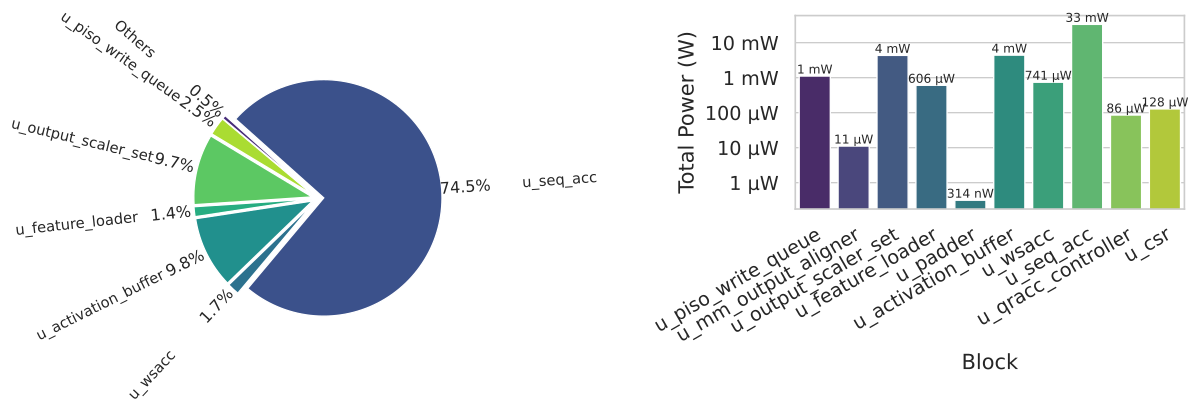
\includegraphics[width=\textwidth]{images/qracc/power_results.png}
    \caption{QRAcc Power Distribution}
    \label{fig:qracc_power_distribution}
\end{figure}

Figure \ref{fig:qracc_power_distribution} shows QRAcc's power distribution. The ACTMEM, being an SRAM bank, consumes a significant amount of power at $4uW$ as expected from memory. Next, the output scalers come at second with $3.6uW$. The output scalers consume power intensely due to having 8-bit multipliers each, and also being the critical path as they're purely combinational required large sizing and thus higher leakage and dynamic energy.  The SeqAcc core consumes the third most power at $1.1uW$ for its digital portion (but in fact, would consume the most power overall due to its analog portions). The main digital contributions to SeqAcc powercomes from the shift-multiplies and having the largest number of internal registers. 

\begin{figure}[htbp]
    \centering
    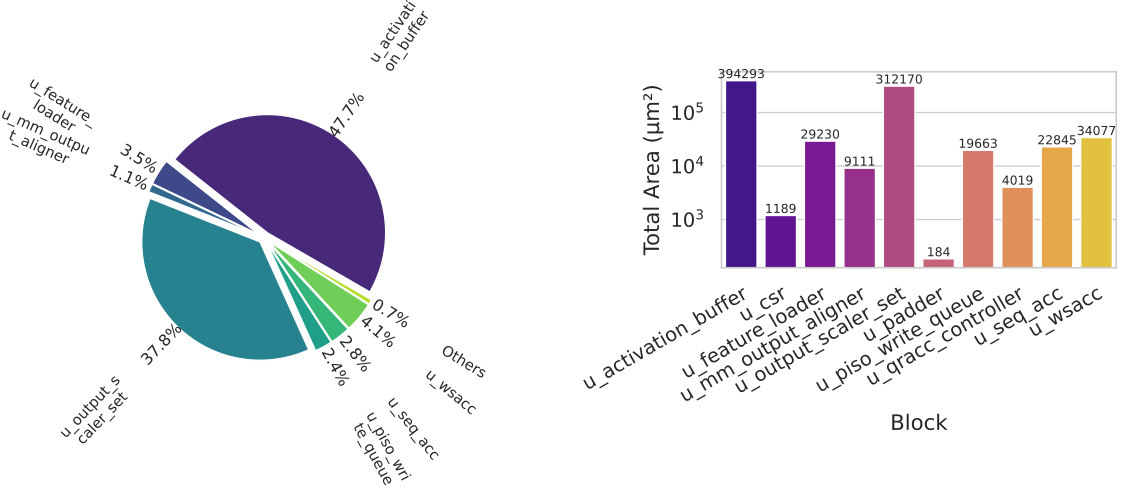
\includegraphics[width=\textwidth]{images/qracc/area_results.png}
    \caption{QRAcc Area Distribution}
    \label{fig:qracc_area_distribution}
\end{figure}

Figure \ref{fig:qracc_area_distribution} shows QRAcc's area distribution. The ACTMEM occupies the most area at $0.39mm^2$ which is due to it being made of 32 banks of $12.23um^2$ 8kB SRAMs. The output scalers come a close second at $0.3mm^2$ due to their utilization of 8b multipliers, barrel shifters, and large number of internal registers (256x32b bias registers, 256x16b scale and shift registers, 256x8b output offset registers). The WSAcc, FL, Write Queues, and SeqAcc all consume in the order of $10-100kum^2$ since they all utilize internal registers- 256x8b for the FL, 256x16b accumulators for the SeqAcc, 32x8b weight registers for WSAcc, and 8x(256+13)b shift registers for the write queues. Barrel shifters and address multiplexing also contribute significant remaining area to the FL, output aligner.

\subsection{State-dependent Power Consumption}

In order to account for an entire power and energy model of QRAcc, we also 
We do this by fully characterizing the state-dependent power consumption results of QRAcc. Table \ref{tab:qracc_state_power} shows the state-dependent power consumption (per Block) of QRAcc. Figure \ref{fig:qracc_state_power} shows the same data in a bar chart. By far, the Compute Analog state consumes the most power at $21.9 \mu W$. Compute Analog consumes this much power mainly due to the full use of the 256 output scaler blocks which are expensive due to their 16x8b array multipliers and barrel shifters. The Compute Digital state comes at second with $10.6 \mu W$, which is expected since it also uses the output scalers and also the WSacc core which also contains 32 8b multipliers.

\begin{table}[]
\centering
\label{tab:qracc_state_power}
\caption{QRAcc State-dependent Power Consumption in W}
\resizebox{\columnwidth}{!}{%
\begin{tabular}{c|rrrrrrrrr|r}
\cline{2-10}
 &
  \multicolumn{9}{c|}{\textbf{State}} &
  \multicolumn{1}{l}{} \\ \hline
\multicolumn{1}{|c|}{\textbf{Module}} &
  \multicolumn{1}{c}{\textbf{\begin{tabular}[c]{@{}c@{}}Compute\\ Analog\end{tabular}}} &
  \multicolumn{1}{c}{\textbf{\begin{tabular}[c]{@{}c@{}}Compute\\ Digital\end{tabular}}} &
  \multicolumn{1}{c}{\textbf{Idle}} &
  \multicolumn{1}{c}{\textbf{\begin{tabular}[c]{@{}c@{}}Load\\ Acts\end{tabular}}} &
  \multicolumn{1}{c}{\textbf{\begin{tabular}[c]{@{}c@{}}Load\\ Bias\end{tabular}}} &
  \multicolumn{1}{c}{\textbf{\begin{tabular}[c]{@{}c@{}}Load \\ Scalers\end{tabular}}} &
  \multicolumn{1}{c}{\textbf{\begin{tabular}[c]{@{}c@{}}Load \\ Weights\end{tabular}}} &
  \multicolumn{1}{c}{\textbf{\begin{tabular}[c]{@{}c@{}}Load \\ Weights \\ (WSAcc)\end{tabular}}} &
  \multicolumn{1}{c|}{\textbf{\begin{tabular}[c]{@{}c@{}}Read \\ Acts\end{tabular}}} &
  \multicolumn{1}{c|}{\textbf{\begin{tabular}[c]{@{}c@{}}Average\\ Power\end{tabular}}} \\ \hline
\multicolumn{1}{|c|}{\begin{tabular}[c]{@{}c@{}}Activation\\ Memory\end{tabular}} &
  \cellcolor[HTML]{FFE59A}4.56E-06 &
  \cellcolor[HTML]{FFE59B}4.44E-06 &
  \cellcolor[HTML]{FFE59D}4.10E-06 &
  \cellcolor[HTML]{FFE59B}4.48E-06 &
  \cellcolor[HTML]{FFE59C}4.31E-06 &
  \cellcolor[HTML]{FFE59C}4.31E-06 &
  \cellcolor[HTML]{FFE59C}4.32E-06 &
  \cellcolor[HTML]{FFE59C}4.29E-06 &
  \cellcolor[HTML]{FFE59B}4.40E-06 &
  \multicolumn{1}{r|}{\cellcolor[HTML]{FFD666}4.36E-06} \\ \cline{1-1}
\multicolumn{1}{|c|}{\begin{tabular}[c]{@{}c@{}}Feature\\ Loader\end{tabular}} &
  \cellcolor[HTML]{FFEBB1}7.61E-07 &
  \cellcolor[HTML]{FFEBB2}6.50E-07 &
  \cellcolor[HTML]{FFF0C4}3.15E-07 &
  \cellcolor[HTML]{FFEFC3}3.21E-07 &
  \cellcolor[HTML]{FFEFC3}3.21E-07 &
  \cellcolor[HTML]{FFEFC3}3.21E-07 &
  \cellcolor[HTML]{FFEFC3}3.21E-07 &
  \cellcolor[HTML]{FFF0C3}3.20E-07 &
  \cellcolor[HTML]{FFEBB3}4.17E-07 &
  \multicolumn{1}{r|}{\cellcolor[HTML]{FFEDB9}4.16E-07} \\ \cline{1-1}
\multicolumn{1}{|c|}{\begin{tabular}[c]{@{}c@{}}Output\\ Aligner\end{tabular}} &
  \cellcolor[HTML]{FFF6DA}1.99E-07 &
  \cellcolor[HTML]{FFFDF5}5.63E-08 &
  \cellcolor[HTML]{FFFBF0}8.32E-08 &
  \cellcolor[HTML]{FFFFFD}1.37E-08 &
  \cellcolor[HTML]{FFFFFD}1.37E-08 &
  \cellcolor[HTML]{FFFFFC}1.65E-08 &
  \cellcolor[HTML]{FFFFFD}1.13E-08 &
  \cellcolor[HTML]{FFFFFD}1.13E-08 &
  \cellcolor[HTML]{FFFFFD}1.37E-08 &
  \multicolumn{1}{r|}{\cellcolor[HTML]{FFFFFF}4.65E-08} \\ \cline{1-1}
\multicolumn{1}{|c|}{\begin{tabular}[c]{@{}c@{}}Output \\ Scaler\end{tabular}} &
  \cellcolor[HTML]{FFD666}1.31E-05 &
  \cellcolor[HTML]{FFE8A5}2.73E-06 &
  \cellcolor[HTML]{FFE8A7}2.41E-06 &
  \cellcolor[HTML]{FFE8A7}2.39E-06 &
  \cellcolor[HTML]{FFE8A8}2.36E-06 &
  \cellcolor[HTML]{FFE8A8}2.37E-06 &
  \cellcolor[HTML]{FFE8A8}2.31E-06 &
  \cellcolor[HTML]{FFE8A8}2.34E-06 &
  \cellcolor[HTML]{FFE8A8}2.35E-06 &
  \multicolumn{1}{r|}{\cellcolor[HTML]{FFDB75}3.60E-06} \\ \cline{1-1}
\multicolumn{1}{|c|}{\begin{tabular}[c]{@{}c@{}}Padding\\ Module\end{tabular}} &
  \cellcolor[HTML]{FFF5D8}2.11E-07 &
  \cellcolor[HTML]{FFF9E6}1.36E-07 &
  \cellcolor[HTML]{FFFFFF}3.26E-10 &
  \cellcolor[HTML]{FFFFFF}5.01E-10 &
  \cellcolor[HTML]{FFFFFF}3.46E-10 &
  \cellcolor[HTML]{FFFFFF}3.46E-10 &
  \cellcolor[HTML]{FFFFFF}3.46E-10 &
  \cellcolor[HTML]{FFFFFF}3.46E-10 &
  \cellcolor[HTML]{FFFBEF}8.74E-08 &
  \multicolumn{1}{r|}{\cellcolor[HTML]{FFFFFF}4.85E-08} \\ \cline{1-1}
\multicolumn{1}{|c|}{\begin{tabular}[c]{@{}c@{}}Write\\ Queue\end{tabular}} &
  \cellcolor[HTML]{FFEBB1}7.76E-07 &
  \cellcolor[HTML]{FFEBB2}6.34E-07 &
  \cellcolor[HTML]{FFEBB3}5.60E-07 &
  \cellcolor[HTML]{FFEBB2}5.69E-07 &
  \cellcolor[HTML]{FFEBB2}5.68E-07 &
  \cellcolor[HTML]{FFEBB2}5.68E-07 &
  \cellcolor[HTML]{FFEBB2}5.68E-07 &
  \cellcolor[HTML]{FFEBB3}5.64E-07 &
  \cellcolor[HTML]{FFEBB2}5.66E-07 &
  \multicolumn{1}{r|}{\cellcolor[HTML]{FFEBB1}5.97E-07} \\ \cline{1-1}
\multicolumn{1}{|c|}{Controller} &
  \cellcolor[HTML]{FFFDF5}5.54E-08 &
  \cellcolor[HTML]{FFFDF6}5.26E-08 &
  \cellcolor[HTML]{FFFDF6}5.07E-08 &
  \cellcolor[HTML]{FFFDF7}4.65E-08 &
  \cellcolor[HTML]{FFFDF7}4.57E-08 &
  \cellcolor[HTML]{FFFDF7}4.57E-08 &
  \cellcolor[HTML]{FFFDF7}4.62E-08 &
  \cellcolor[HTML]{FFFDF7}4.55E-08 &
  \cellcolor[HTML]{FFFDF7}4.59E-08 &
  \multicolumn{1}{r|}{\cellcolor[HTML]{FFFFFF}4.82E-08} \\ \cline{1-1}
\multicolumn{1}{|c|}{\begin{tabular}[c]{@{}c@{}}SeqAcc\\ (Digital)\end{tabular}} &
  \cellcolor[HTML]{FFE9AB}1.83E-06 &
  \cellcolor[HTML]{FFEAB0}1.02E-06 &
  \cellcolor[HTML]{FFEBB0}1.00E-06 &
  \cellcolor[HTML]{FFEAB0}1.01E-06 &
  \cellcolor[HTML]{FFEAB0}1.01E-06 &
  \cellcolor[HTML]{FFEAB0}1.01E-06 &
  \cellcolor[HTML]{FFEAB0}1.02E-06 &
  \cellcolor[HTML]{FFEAB0}1.01E-06 &
  \cellcolor[HTML]{FFEAB0}1.01E-06 &
  \multicolumn{1}{r|}{\cellcolor[HTML]{FFE8A7}1.10E-06} \\ \cline{1-1}
\multicolumn{1}{|c|}{WSAcc} &
  \cellcolor[HTML]{FFEBB3}4.01E-07 &
  \cellcolor[HTML]{FFEBB0}9.00E-07 &
  \cellcolor[HTML]{FFEDB9}3.73E-07 &
  \cellcolor[HTML]{FFECB5}3.91E-07 &
  \cellcolor[HTML]{FFECB6}3.89E-07 &
  \cellcolor[HTML]{FFECB6}3.89E-07 &
  \cellcolor[HTML]{FFECB6}3.89E-07 &
  \cellcolor[HTML]{FFEBB3}4.01E-07 &
  \cellcolor[HTML]{FFECB4}3.98E-07 &
  \multicolumn{1}{r|}{\cellcolor[HTML]{FFEBB3}4.48E-07} \\ \hline
\multicolumn{1}{|c|}{\begin{tabular}[c]{@{}c@{}}Total\\ Power\end{tabular}} &
  \cellcolor[HTML]{FFD666}2.19E-05 &
  \cellcolor[HTML]{FFE9AA}1.06E-05 &
  \cellcolor[HTML]{FFFFFF}8.89E-06 &
  \cellcolor[HTML]{FFEBB2}9.22E-06 &
  \cellcolor[HTML]{FFEDBB}9.02E-06 &
  \cellcolor[HTML]{FFEBB3}9.03E-06 &
  \cellcolor[HTML]{FFF2CC}8.99E-06 &
  \cellcolor[HTML]{FFF2CE}8.98E-06 &
  \cellcolor[HTML]{FFEBB2}9.29E-06 &
  \multicolumn{1}{r|}{1.07E-05} \\ \hline
\end{tabular}%
}
\end{table}

\begin{figure}[htbp]
    \centering
    \includegraphics[width=\textwidth]{images/qracc/state_power_consumption.png}
    \caption{QRAcc Per-state Power Consumption}
    \label{fig:qracc_state_power}
\end{figure}

\section{Conclusion}

In this chapter, we presented QRAcc, a charge-redistribution SRAM-based AIMC accelerator for DNNs. QRAcc is a fully integrated AIMC accelerator that can perform both analog and digital computations. It uses SeqAcc as its main analog core and WSAcc as its digital core. QRAcc achieves a peak energy efficiency of 516.1 TOPS/W at 409.6 GOPS, which is comparable to state-of-the-art.

In the next chapter, we will present the results of optimizing DNN mappings on QRAcc with MARP.